\documentclass[11pt,a4paper]{article}

% --- Kodowanie i język ---
\usepackage[utf8]{inputenc}
\usepackage[T1]{fontenc}
\usepackage[polish]{babel}
\usepackage{lmodern}

% --- Grafika, tabele, matematyka ---
\usepackage{graphicx}
\usepackage{float}
\usepackage{booktabs}
\usepackage{array}
\usepackage{amsmath}
\usepackage{amssymb}
\usepackage{caption}
\usepackage{subcaption}
\usepackage{xcolor}
\usepackage{enumitem}

% --- Listingi kodu ---
\usepackage{listings}

% --- Hiperłącza (na końcu preambuły) ---
\usepackage[hidelinks]{hyperref}

\graphicspath{{rysunki/}}

% --- Konfiguracja listingów (z obsługą polskich znaków) ---
\definecolor{codegray}{rgb}{0.5,0.5,0.5}
\definecolor{codegreen}{rgb}{0,0.5,0}
\definecolor{codeblue}{rgb}{0.1,0.1,0.6}
\definecolor{codebg}{rgb}{0.97,0.97,0.97}

\lstset{
  basicstyle=\ttfamily\footnotesize,
  backgroundcolor=\color{codebg},
  commentstyle=\color{codegreen},
  keywordstyle=\color{codeblue}\bfseries,
  stringstyle=\color{red!60!black},
  numberstyle=\tiny\color{codegray},
  numbers=left,
  numbersep=8pt,
  breaklines=true,
  breakatwhitespace=true,
  frame=single,
  rulecolor=\color{gray!40},
  showstringspaces=false,
  tabsize=4,
  captionpos=b,
  inputencoding=utf8,
  extendedchars=true,
  literate=%
    {ą}{{\k{a}}}1 {ć}{{\'c}}1 {ę}{{\k{e}}}1 {ł}{{\l}}1 {ń}{{\'n}}1
    {ó}{{\'o}}1 {ś}{{\'s}}1 {ź}{{\'z}}1 {ż}{{\.z}}1
    {Ą}{{\k{A}}}1 {Ć}{{\'C}}1 {Ę}{{\k{E}}}1 {Ł}{{\L}}1 {Ń}{{\'N}}1
    {Ó}{{\'O}}1 {Ś}{{\'S}}1 {Ź}{{\'Z}}1 {Ż}{{\.Z}}1
}

\lstdefinestyle{py}{language=Python}
\lstdefinestyle{cpp}{language=C++}

% Pozwala TeX-owi nieco rozciągnąć wiersze, ograniczając "overfull hbox".
\emergencystretch=3em

\begin{document}

% =====================================================================
\begin{titlepage}
\centering
\vspace*{2cm}
{\Large\bfseries Projekt z uczenia maszynowego\par}
\vspace{1.5cm}
{\Huge\bfseries Nauczenie komputera sterowania\\[0.3cm] samochodem w grze 2D\par}
\vspace{0.8cm}
{\large Sieć neuronowa jako kierowca pojazdu sterowanego\\ na podstawie sygnałów z czujników odległości\par}
\vspace{2.5cm}
{\large Raport końcowy\par}
\vfill
{\large \today\par}
\end{titlepage}

\tableofcontents
\newpage

% =====================================================================
\section{Cel projektu}
\label{sec:cel}

Celem projektu jest \textbf{nauczenie komputera samodzielnego sterowania samochodem
w grze 2D}. Zadaniem wytrenowanego modelu jest obserwowanie stanu pojazdu i jego
otoczenia, a następnie podejmowanie w czasie rzeczywistym decyzji sterujących
(przyspieszanie, hamowanie, skręt w lewo, skręt w prawo) tak, aby pojazd poruszał
się po torze i dojechał do mety, nie uderzając w przeszkody.

Należy podkreślić, że \emph{właściwym celem projektu nie jest samo testowanie
wartości hiperparametrów}. Strojenie konfiguracji modelu (rozdział~\ref{sec:strojenie})
jest jedynie \textbf{środkiem} prowadzącym do celu nadrzędnego --- uzyskania modelu,
który skutecznie zastępuje człowieka przy kierownicy. Eksperymenty z hiperparametrami
traktujemy więc jako narzędzie poprawiające jakość kierowcy, a nie jako produkt sam
w sobie.

Projekt obejmuje pełny proces uczenia maszynowego:
\begin{enumerate}[noitemsep]
  \item zebranie danych z gry (rozgrywka człowieka jako wzorzec),
  \item przygotowanie i normalizację danych,
  \item analizę eksploracyjną zebranego zbioru,
  \item zaprojektowanie i wytrenowanie sieci neuronowej,
  \item wyznaczenie modelu bazowego i jego optymalizację,
  \item ocenę modelu metrykami klasyfikacji,
  \item wdrożenie modelu w grze i sterowanie pojazdem w czasie rzeczywistym.
\end{enumerate}

% =====================================================================
\section{Wykorzystany model uczenia maszynowego}
\label{sec:model-overview}

W projekcie kierowcę-komputer realizuje \textbf{sztuczna sieć neuronowa typu
wielowarstwowy perceptron} (ang. \emph{multilayer perceptron}, MLP; sieć
jednokierunkowa, \emph{feedforward}). Jest to model uczenia nadzorowanego, który
odwzorowuje wektor cech opisujący sytuację na torze na wektor decyzji sterujących.

\subsection{Idea modelu}

Sieć złożona jest z kolejnych \emph{warstw gęstych} (w pełni połączonych). Każdy
neuron warstwy oblicza ważoną sumę swoich wejść powiększoną o wyraz wolny (\emph{bias}),
a wynik przepuszcza przez nieliniową funkcję aktywacji. Dla $l$-tej warstwy:
\begin{equation}
\mathbf{h}^{(l)} = \phi\!\left(\mathbf{W}^{(l)}\mathbf{h}^{(l-1)} + \mathbf{b}^{(l)}\right),
\qquad \mathbf{h}^{(0)} = \mathbf{x},
\label{eq:forward}
\end{equation}
gdzie $\mathbf{x}\in\mathbb{R}^{81}$ to wektor cech wejściowych (rozdział~\ref{sec:problem}),
$\mathbf{W}^{(l)}$ i $\mathbf{b}^{(l)}$ to wagi i biasy uczone podczas treningu, a
$\phi$ to funkcja aktywacji (w naszym przypadku ReLU). Warstwa wyjściowa jest
\emph{liniowa} (bez aktywacji) i zwraca cztery \emph{logity}
$\mathbf{z}=(z_\text{acc}, z_\text{brake}, z_\text{left}, z_\text{right})\in\mathbb{R}^4$,
zamieniane na prawdopodobieństwa funkcją sigmoidalną (rozdział~\ref{sec:strata}).
Uczenie polega na takim doborze wag $\mathbf{W}^{(l)}, \mathbf{b}^{(l)}$ (metodą
spadku gradientu i propagacji wstecznej), aby minimalizować funkcję straty.

\subsection{Uzasadnienie wyboru}

MLP dobrze pasuje do tego zadania, ponieważ:
\begin{itemize}[noitemsep]
  \item wejście ma \textbf{stałą długość} (81 cech) i postać tabelaryczną, bez
        struktury przestrzennej czy sekwencyjnej, która uzasadniałaby sieci
        splotowe (CNN) lub rekurencyjne (RNN);
  \item wnioskowanie jest \textbf{bardzo szybkie}, co jest kluczowe przy
        sterowaniu w czasie rzeczywistym (predykcja w każdej klatce gry);
  \item model ma wystarczającą pojemność, by uchwycić nieliniowe zależności między
        odczytami czujników a decyzjami kierowcy.
\end{itemize}
Szczegółową architekturę konkretnej sieci (\texttt{DriverNet}) opisano w
rozdziale~\ref{sec:model}, a teorię użytych w niej mechanizmów --- w
rozdziale~\ref{sec:teoria-warstw}.

% =====================================================================
\section{Opis środowiska --- gra w C++}
\label{sec:srodowisko}

Środowiskiem projektu jest autorska gra napisana w języku C++ z wykorzystaniem
biblioteki graficznej \texttt{raylib}. Gra przedstawia jazdę samochodem w widoku
z góry (2D). Gracz buduje tor z klocków (linie barierowe, filary, zakręty oraz
bloki typu start/meta/checkpoint), a następnie steruje pojazdem.

\subsection{Model fizyki pojazdu}

Pojazd opisany jest położeniem, kątem obrotu oraz prędkością skalarną. Sterowanie
odbywa się czterema niezależnymi sygnałami (\emph{Controls}): \texttt{accelerate},
\texttt{brake}, \texttt{steerLeft}, \texttt{steerRight}. Uproszczona dynamika
(z pliku \texttt{Car.cpp}) zakłada m.in. naturalne tłumienie prędkości, ograniczenie
prędkości do przedziału $[-5, 10]$ oraz zależność siły skrętu od prędkości:

\noindent\begin{minipage}{\linewidth}
\begin{lstlisting}[style=cpp,caption={Aktualizacja prędkości i obrotu pojazdu (fragment \texttt{Car.cpp}).}]
void Car::updateSpeedRot(Controls inputs) {
    this->speed *= 0.995f;                 // naturalne tlumienie
    if (inputs.accelerate && this->speed < 10) this->speed += 0.1f;
    if (inputs.brake      && this->speed > -5) this->speed -= 0.3f;
    // ... ograniczenie predkosci do [-5, 10] ...

    // sila skretu (turnSpeed) zalezy od aktualnej predkosci
    float turnSpeed = /* funkcja predkosci, maxTurn = 3.0f */;
    if (inputs.steerLeft)  this->rotation -= turnSpeed;
    if (inputs.steerRight) this->rotation += turnSpeed;
}
\end{lstlisting}
\end{minipage}

Kolizja z barierą (typ~0) powoduje reset pojazdu do punktu odrodzenia, blok
checkpoint (typ~2) aktualizuje punkt odrodzenia, a wjazd na metę (typ~3) zatrzymuje
licznik czasu i kończy przejazd.

\subsection{Czujniki --- ,,oczy'' kierowcy}
\label{sec:czujniki}

Postrzeganie otoczenia przez pojazd zrealizowano za pomocą \textbf{20 promieni
(raycastów)} rozchodzących się od środka samochodu. Trzynaście promieni pokrywa
przedni wachlarz (co $10^\circ$), a kolejnych siedem obserwuje tył i boki. Dla
każdego promienia wyznaczana jest:
\begin{itemize}[noitemsep]
  \item \textbf{odległość} do najbliższego trafionego obiektu (\texttt{ray\_dist}),
  \item \textbf{typ} trafionego obiektu (\texttt{ray\_type}): $-1$ --- brak trafienia,
        $0$ --- ściana/przeszkoda, $1$ --- meta.
\end{itemize}

Te 20 odległości oraz 20 typów wraz z prędkością tworzą pełny \emph{stan gry}
(\texttt{GameState}), który stanowi wejście modelu. Zestaw promieni jest aktualizowany
względem aktualnego obrotu pojazdu:

\noindent\begin{minipage}{\linewidth}
\begin{lstlisting}[style=cpp,caption={Wyznaczanie kierunków promieni (fragment \texttt{Car.cpp}).}]
void Car::UpdateRays() {
    // 13 promieni - przedni wachlarz (co 10 stopni)
    for (int i = 0; i < 13; i++)
        this->Rays[i] = { cos((-60 + 10*i + this->rotation)*DEG2RAD),
                          sin((-60 + 10*i + this->rotation)*DEG2RAD) };
    // 7 promieni - tyl i boki (co 30 stopni)
    for (int i = 0; i < 7; i++)
        this->Rays[i+13] = { /* analogicznie: 100 + 30*i + rotation */ };
}
\end{lstlisting}
\end{minipage}

\subsection{Zbieranie danych}

Podczas jazdy sterowanej przez człowieka gra zapisuje do pliku CSV kolejne stany
gry razem z wciśniętymi w danej klatce klawiszami. Nagłówek pliku generowany jest
w \texttt{GameState.cpp} i ma postać:
\[
\texttt{car\_speed},\ \texttt{ray\_dist\_0},\ \texttt{ray\_type\_0},\ \dots,\
\texttt{ray\_dist\_19},\ \texttt{ray\_type\_19},
\]
\[
\texttt{accelerate},\ \texttt{brake},\ \texttt{steer\_left},\ \texttt{steer\_right}.
\]
W ten sposób człowiek pełni rolę ,,nauczyciela'': model uczy się odwzorowywać
decyzje gracza w zależności od sytuacji na torze (uczenie nadzorowane, ang.
\emph{imitation learning}).

Dane wykorzystane w projekcie zostały zebrane przez \textbf{jednego gracza} na
\textbf{czterech różnych torach}. Łączny zarejestrowany materiał odpowiada około
\textbf{10 minutom jazdy}.

% =====================================================================
\section{Sformułowanie problemu uczenia maszynowego}
\label{sec:problem}

Zadanie sterowania pojazdem sprowadzono do \textbf{klasyfikacji wieloetykietowej}
(ang. \emph{multi-label classification}). Dla danego stanu $\mathbf{x}$ model
przewiduje cztery niezależne prawdopodobieństwa odpowiadające czterem klawiszom
sterującym:
\[
\hat{\mathbf{y}} = \big(p_\text{acc},\ p_\text{brake},\ p_\text{left},\ p_\text{right}\big),
\qquad p_k \in (0,1).
\]
Etykiety nie są wzajemnie wykluczające się (np. można jednocześnie przyspieszać i
skręcać), dlatego nie jest to klasyczna klasyfikacja jednoklasowa, lecz cztery
sprzężone problemy binarne uczone wspólną siecią.

\subsection{Cechy wejściowe}

Wejście modelu budowane jest identycznie po stronie Pythona (uczenie) i C++
(wnioskowanie w grze). Składa się z \textbf{81 cech}:
\begin{itemize}[noitemsep]
  \item 1 cecha numeryczna: \texttt{car\_speed},
  \item 20 cech numerycznych: \texttt{ray\_dist\_0..19},
  \item 60 cech binarnych: zakodowanie ,,one-hot'' typu każdego z 20 promieni
        (3 możliwe wartości: $-1$, $0$, $1$).
\end{itemize}
Cechy numeryczne (\texttt{car\_speed} oraz odległości) są standaryzowane
(rozdział~\ref{sec:przygotowanie}), natomiast cechy typu promienia, jako zmienne
kategoryczne, kodowane są binarnie bez skalowania.

\subsection{Funkcja straty i nierównowaga klas}
\label{sec:strata}

\paragraph{Sigmoida i entropia krzyżowa.}
Każdy logit $z_k$ zamieniany jest na prawdopodobieństwo funkcją sigmoidalną
$\sigma(z) = 1/(1 + e^{-z}) \in (0,1)$, osobną dla każdej z czterech akcji (co
odróżnia klasyfikację wieloetykietową od jednoklasowej z funkcją \emph{softmax}).
Funkcją straty dla pojedynczej etykiety $y\in\{0,1\}$ przy $p=\sigma(z)$ jest
binarna entropia krzyżowa (BCE):
\begin{equation}
\ell(y, p) = -\big[\,y\,\log p + (1-y)\,\log(1-p)\,\big].
\label{eq:bce}
\end{equation}
W praktyce stosujemy \texttt{BCEWithLogitsLoss}, które liczy stratę bezpośrednio
z logitu $z$ (numerycznie stabilnie, bez osobnego nakładania sigmoidy w treningu).

\paragraph{Ważenie klasy pozytywnej.}
Ponieważ klawisze sterujące występują z bardzo różną częstością (hamowanie jest
rzadkie, a przyspieszanie niemal stałe), do każdej etykiety przypisano wagę klasy
pozytywnej $w_k$ (\texttt{pos\_weight}), która wzmacnia wkład rzadkich, lecz
istotnych przykładów pozytywnych:
\begin{equation}
\ell_{w}(y, z) = -\big[\,w\,y\,\log\sigma(z) + (1-y)\,\log(1-\sigma(z))\,\big].
\label{eq:wbce}
\end{equation}
Wagę dobiera się na podstawie proporcji liczby przykładów negatywnych do
pozytywnych, z ograniczeniem do przedziału $[0{,}5, c]$:
\begin{equation}
w_k = \mathrm{clip}\!\left(\frac{N_\text{neg}^{(k)}}{\max(N_\text{pos}^{(k)},\,1)},\ 0{,}5,\ c\right),
\label{eq:posweight}
\end{equation}
gdzie $c$ to górne ograniczenie (hiperparametr \texttt{pos\_weight\_cap}).
Mechanizm ten zapobiega ignorowaniu rzadkich akcji (np. hamowania).

\paragraph{Strata całkowita.}
Ostateczna strata minimalizowana podczas treningu to średnia
\eqref{eq:wbce} po wszystkich $K=4$ etykietach i $N$ przykładach w paczce:
\begin{equation}
\mathcal{L} = \frac{1}{N\,K}\sum_{i=1}^{N}\sum_{k=1}^{K}
\ell_{w_k}\!\big(y_{ik}, z_{ik}\big).
\label{eq:total-loss}
\end{equation}

% =====================================================================
\section{Dane i ich przygotowanie}
\label{sec:przygotowanie}

\subsection{Charakterystyka zbioru}

Surowy zbiór (\texttt{GameStatesTable.csv}) zawiera ponad $65\,000$ wierszy
zarejestrowanych w trakcie rozgrywki. Każdy wiersz to jedna klatka gry: stan
czujników oraz odpowiadające mu decyzje gracza.

\subsection{Kroki przygotowania danych}

Skrypt przygotowujący dane (zaimplementowany w funkcjach \texttt{load\_data} oraz
\texttt{build\_features}) wykonuje następujące operacje:
\begin{enumerate}[noitemsep]
  \item wczytanie pliku CSV i oczyszczenie nazw kolumn,
  \item konwersję kolumn na typ numeryczny i usunięcie wierszy z brakami
        (\texttt{NaN}), co chroni m.in. przed przypadkowym powtórzeniem nagłówka,
  \item binaryzację etykiet do wartości $\{0,1\}$ progiem $0{,}5$,
  \item opcjonalne usunięcie duplikatów oraz początkowych ,,bezczynnych'' klatek
        (gdy pojazd stoi i nie ma żadnego wejścia),
  \item standaryzację cech numerycznych za pomocą \texttt{StandardScaler}
        (dopasowanego wyłącznie na zbiorze treningowym),
  \item kodowanie one-hot typów promieni,
  \item złączenie cech w macierz $\mathbf{X}$ o 81 kolumnach oraz wektor etykiet
        $\mathbf{y}$ o 4 kolumnach.
\end{enumerate}

\paragraph{Standaryzacja cech (z-score).}
Cechy numeryczne mają różne zakresy (prędkość rzędu jednostek, odległości promieni
rzędu setek), co utrudnia uczenie sieci. Standaryzacja sprowadza każdą cechę do
średniej~$0$ i odchylenia standardowego~$1$:
\begin{equation}
x' = \frac{x - \mu}{\sigma},
\label{eq:standaryzacja}
\end{equation}
gdzie $\mu$ i $\sigma$ to średnia i odchylenie standardowe danej cechy. Co istotne,
parametry te wyznacza się \textbf{wyłącznie na zbiorze treningowym}, a następnie tymi
samymi wartościami przekształca zbiór walidacyjny --- zapobiega to wyciekowi
informacji ze zbioru testowego do procesu uczenia. Cechy kategoryczne (typ promienia)
nie są skalowane, lecz kodowane binarnie (one-hot).

\noindent\begin{minipage}{\linewidth}
\begin{lstlisting}[style=py,caption={Budowa cech wejściowych: standaryzacja liczb i one-hot typów (fragment \texttt{train\_driver\_model.py}).}]
def build_features(df, scaler=None, fit_scaler=False):
    numeric = df[NUMERIC_COLS].astype(np.float32).to_numpy()
    if fit_scaler:                       # scaler dopasowany tylko na zbiorze treningowym
        scaler = StandardScaler()
        numeric = scaler.fit_transform(numeric).astype(np.float32)
    else:
        numeric = scaler.transform(numeric).astype(np.float32)

    type_features = []                   # one-hot typu promienia (kolejnosc: -1, 0, 1)
    for col in TYPE_COLS:
        values = df[col].astype(int).to_numpy()
        for ray_type in RAY_TYPE_VALUES:
            type_features.append((values == ray_type).astype(np.float32).reshape(-1, 1))

    x = np.concatenate([numeric] + type_features, axis=1).astype(np.float32)
    return x, scaler
\end{lstlisting}
\end{minipage}

\subsection{Spójność uczenia i wdrożenia}

Aby model wytrenowany w Pythonie działał identycznie w grze C++, parametry
standaryzacji (średnia i odchylenie) są eksportowane do nagłówka C++
(\texttt{AIScalerData.h}). Dzięki temu funkcja \texttt{BuildAIInputFromGameState}
buduje wektor wejściowy w dokładnie tej samej kolejności i skali co skrypt uczący:

\noindent\begin{minipage}{\linewidth}
\begin{lstlisting}[style=cpp,caption={Standaryzacja cech po stronie gry (fragment \texttt{AIInputBuilder.cpp}).}]
static float ScaleNumericInput(float value, int index) {
    return (value - AI_INPUT_MEAN[index]) / AI_INPUT_SCALE[index];
}
// 1x car_speed + 20x ray_dist + 20x one-hot(ray_type) => 81 cech
\end{lstlisting}
\end{minipage}

% =====================================================================
\section{Analiza eksploracyjna danych}
\label{sec:eda}

\subsection{Rozkład etykiet i nierównowaga klas}

Analiza częstości wciśnięć klawiszy ujawnia silną \textbf{nierównowagę klas}.
Przyspieszanie jest akcją dominującą, natomiast hamowanie pojawia się sporadycznie.
Najlepiej obrazuje to wyznaczony wektor \texttt{pos\_weight}
(rysunek~\ref{fig:posweight}): waga dla hamowania osiąga górny limit ($20$), co
oznacza, że bez korekty sieć ignorowałaby tę akcję. Skręty mają wagi rzędu $4$--$5$,
a przyspieszanie wagę poniżej~$1$ (klasa większościowa).

\begin{figure}[H]
  \centering
  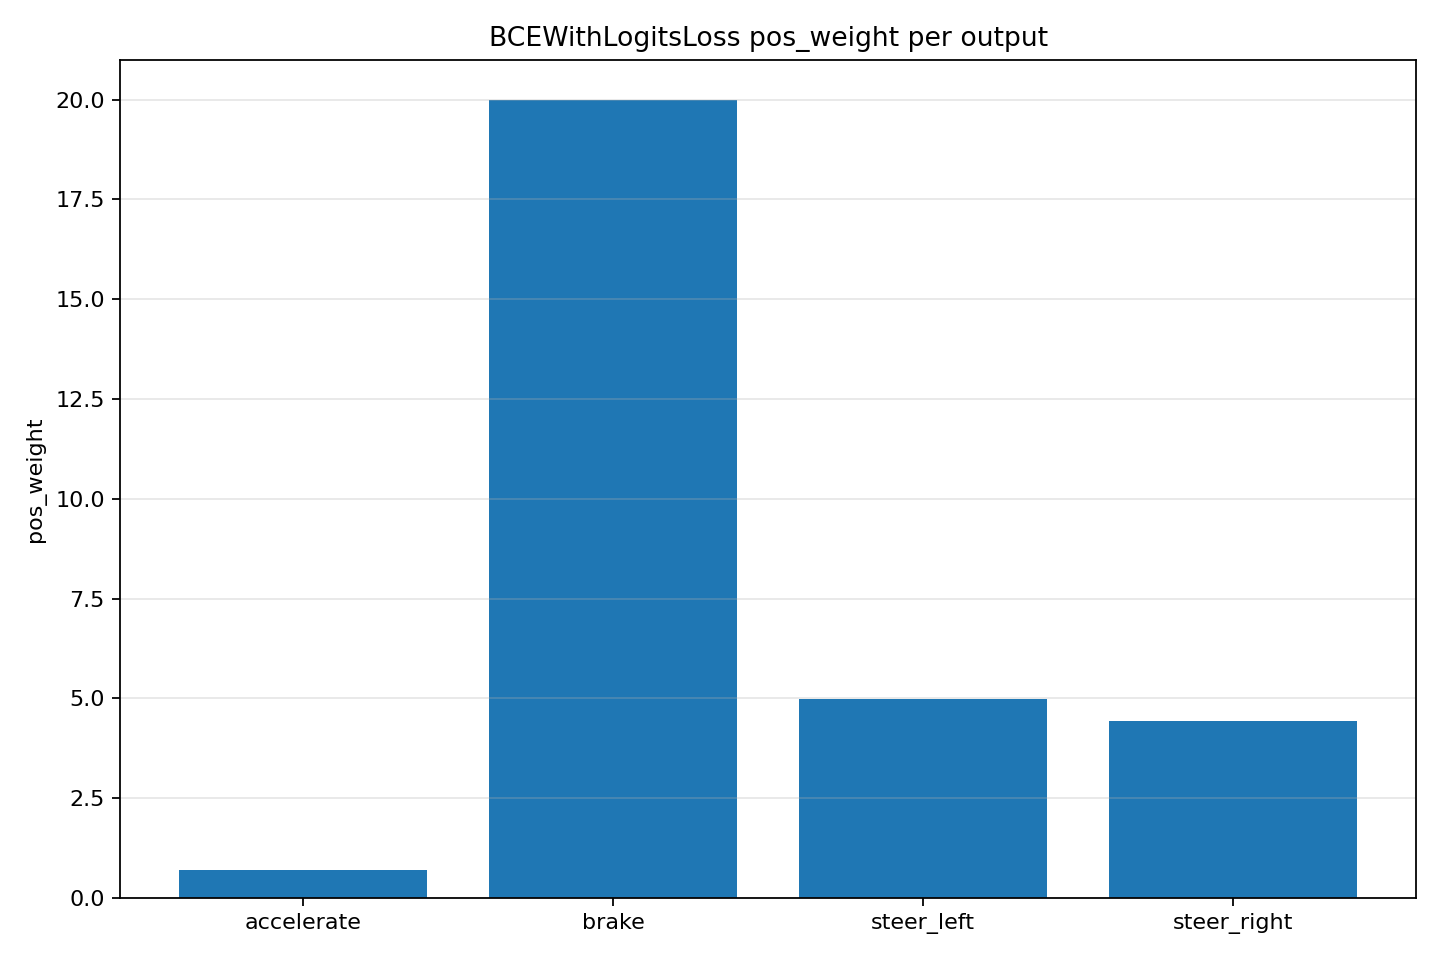
\includegraphics[width=0.7\linewidth]{pos_weight.png}
  \caption{Wagi klasy pozytywnej (\texttt{pos\_weight}) dla poszczególnych akcji.
  Bardzo wysoka waga hamowania odzwierciedla jego rzadkość w danych.}
  \label{fig:posweight}
\end{figure}

\subsection{Wnioski z analizy zbalansowania}

Z powodu nierównowagi klas \textbf{sama dokładność (accuracy) jest metryką mylącą}:
model przewidujący zawsze ,,brak hamowania'' osiągnąłby wysoką trafność dla tej
etykiety, będąc bezużytecznym. Dlatego w ocenie modelu (rozdział~\ref{sec:wyniki})
posługujemy się dodatkowo precyzją, czułością oraz miarą F1 liczonymi osobno dla
każdej akcji, ze szczególnym uwzględnieniem hamowania. Z tego samego powodu w treningu
zastosowano ważenie klas oraz strojenie progów decyzyjnych.

% =====================================================================
\section{Architektura modelu}
\label{sec:model}

Wybranym modelem jest \textbf{wielowarstwowy perceptron} (MLP) zaimplementowany
w bibliotece PyTorch (klasa \texttt{DriverNet}). Sieć przyjmuje 81 cech i zwraca
4 logity. W wariancie podstawowym wykorzystano normalizację wsadową
(\emph{batch normalization}), funkcje aktywacji ReLU oraz warstwę dropout
przeciwdziałającą przeuczeniu.

\noindent\begin{minipage}{\linewidth}
\begin{lstlisting}[style=py,caption={Architektura sieci \texttt{DriverNet} (fragment \texttt{grid\_search\_driver\_basic.py}). Liczba i rozmiary warstw ukrytych są strojonym hiperparametrem.}]
class DriverNet(nn.Module):
    def __init__(self, input_size: int, dropout: float):
        super().__init__()
        self.net = nn.Sequential(
            nn.Linear(input_size, 128),
            nn.BatchNorm1d(128), nn.ReLU(), nn.Dropout(dropout),
            # ... kolejne warstwy ukryte (Linear + ReLU [+ Dropout]) ...
            nn.Linear(64, 4),     # warstwa wyjsciowa: 4 logity (acc, brake, left, right)
        )
    def forward(self, x):
        return self.net(x)
\end{lstlisting}
\end{minipage}

Sieć zwraca logity (bez sigmoidy), ponieważ funkcja straty
\texttt{BCE\allowbreak WithLogitsLoss} łączy w sobie sigmoidę i entropię krzyżową
w sposób numerycznie stabilny. Sigmoida nakładana jest dopiero na etapie wnioskowania.

\subsection{Teoria użytych mechanizmów}
\label{sec:teoria-warstw}

Architektura \texttt{DriverNet} składa się z kilku typów warstw, których działanie
opisano poniżej.

\paragraph{Warstwa liniowa (\texttt{nn.Linear}).}
Realizuje przekształcenie afiniczne $\mathbf{y} = \mathbf{W}\mathbf{x} + \mathbf{b}$
(por.\ wzór~\eqref{eq:forward}). Macierz wag $\mathbf{W}$ i wektor biasów
$\mathbf{b}$ to parametry uczone. Same warstwy liniowe potrafią modelować tylko
zależności liniowe, dlatego przeplata się je nieliniowymi aktywacjami.

\paragraph{Aktywacja ReLU.}
Funkcja \emph{rectified linear unit} wprowadza nieliniowość:
\begin{equation}
\mathrm{ReLU}(x) = \max(0, x).
\label{eq:relu}
\end{equation}
Jest tania obliczeniowo, a jej gradient (równy $0$ dla $x<0$ i $1$ dla $x>0$)
nie zanika dla dużych wartości dodatnich, co przyspiesza uczenie głębokich sieci.

\paragraph{Normalizacja wsadowa (\texttt{BatchNorm1d}).}
Dla każdej cechy normalizuje aktywacje w obrębie paczki danych, a następnie skaluje
je uczonymi parametrami $\gamma$ i $\beta$:
\begin{equation}
\hat{x} = \frac{x - \mu_{\mathcal{B}}}{\sqrt{\sigma_{\mathcal{B}}^2 + \varepsilon}},
\qquad y = \gamma\,\hat{x} + \beta,
\label{eq:batchnorm}
\end{equation}
gdzie $\mu_{\mathcal{B}}$, $\sigma_{\mathcal{B}}^2$ to średnia i wariancja cechy
w paczce, a $\varepsilon$ to mała stała zapewniająca stabilność. Normalizacja
stabilizuje rozkład aktywacji i pozwala na szybsze, stabilniejsze uczenie.
Dodatkowo, jako technikę regularyzacji, architektura może wykorzystywać warstwy
\emph{dropout} losowo wyłączające część neuronów podczas treningu (siła dropoutu
jest jednym ze strojonych hiperparametrów).

% =====================================================================
\section{Metodyka eksperymentów}
\label{sec:metodyka}

\subsection{Podział danych i powtarzalność}

Zbiór dzielony jest na część treningową i walidacyjną (domyślnie $80/20$).
Gdy w danych dostępna jest kolumna identyfikująca przejazd (\texttt{episode\_id}),
podział wykonywany jest \emph{grupowo} (całe przejazdy trafiają do jednego zbioru),
co zapobiega wyciekowi informacji między klatkami tego samego przejazdu i daje
uczciwszą ocenę. Powtarzalność zapewnia ustalone ziarno losowości
(\texttt{set\_seed}) dla bibliotek \texttt{random}, \texttt{numpy} i \texttt{torch}.

\subsection{Procedura treningu}

Trening wykorzystuje optymalizator \texttt{AdamW} oraz mechanizm \textbf{wczesnego
zatrzymania} (\emph{early stopping}).

\paragraph{Optymalizator AdamW.}
Wagi aktualizowane są metodą gradientową z adaptacyjnym krokiem (Adam) i
\emph{odsprzężoną} regularyzacją wag (\emph{weight decay}). Dla gradientu
$\mathbf{g}_t$ utrzymywane są wykładnicze średnie pierwszego i drugiego momentu:
\begin{align}
\mathbf{m}_t &= \beta_1 \mathbf{m}_{t-1} + (1-\beta_1)\,\mathbf{g}_t, &
\hat{\mathbf{m}}_t &= \frac{\mathbf{m}_t}{1-\beta_1^{\,t}}, \\
\mathbf{v}_t &= \beta_2 \mathbf{v}_{t-1} + (1-\beta_2)\,\mathbf{g}_t^{2}, &
\hat{\mathbf{v}}_t &= \frac{\mathbf{v}_t}{1-\beta_2^{\,t}},
\end{align}
a aktualizacja parametrów ma postać:
\begin{equation}
\boldsymbol{\theta}_t = \boldsymbol{\theta}_{t-1}
- \eta\left(\frac{\hat{\mathbf{m}}_t}{\sqrt{\hat{\mathbf{v}}_t}+\varepsilon}
+ \lambda\,\boldsymbol{\theta}_{t-1}\right),
\label{eq:adamw}
\end{equation}
gdzie $\eta$ to współczynnik uczenia, $\lambda$ to siła regularyzacji
(\texttt{weight\_decay}), a $\beta_1, \beta_2$ to współczynniki wygładzania momentów.
Składnik $\lambda\,\boldsymbol{\theta}_{t-1}$ ,,ściąga'' wagi w stronę zera,
ograniczając przeuczenie. W odróżnieniu od klasycznego Adama z regularyzacją L2,
AdamW odsprzęga ten składnik od adaptacyjnego skalowania, co poprawia generalizację.

\paragraph{Wczesne zatrzymanie.}
Zapamiętywany jest stan modelu o najmniejszej stracie walidacyjnej, a uczenie
przerywane jest, gdy strata nie poprawia się przez ustaloną liczbę epok
(\texttt{patience}). Chroni to przed przeuczeniem i skraca czas treningu.

\subsection{Metryki oceny}

Ze względu na nierównowagę klas oraz wieloetykietowy charakter problemu raportowane
są poniższe metryki. Oznaczmy przez TP, FP, FN, TN odpowiednio liczbę trafień
prawdziwie/fałszywie dodatnich i fałszywie/prawdziwie ujemnych.

\paragraph{Precyzja, czułość i F1.}
Precyzja mówi, jaka część przewidzianych ,,wciśnięć'' była trafna, a czułość
(\emph{recall}) --- jaką część rzeczywistych wciśnięć udało się wykryć:
\begin{equation}
\mathrm{Precyzja} = \frac{TP}{TP+FP},\qquad
\mathrm{Czu\l{}o\'s\'c} = \frac{TP}{TP+FN}.
\label{eq:prec-rec}
\end{equation}
Miara F1 to ich średnia harmoniczna, równoważąca oba aspekty --- szczególnie
przydatna przy nierównowadze klas:
\begin{equation}
F_1 = \frac{2\cdot\mathrm{Precyzja}\cdot\mathrm{Czu\l{}o\'s\'c}}
{\mathrm{Precyzja}+\mathrm{Czu\l{}o\'s\'c}}.
\label{eq:f1}
\end{equation}
\emph{Macro-F1} to średnia $F_1$ po wszystkich $K=4$ akcjach (każda akcja waży tak
samo, niezależnie od częstości): $\mathrm{macro\text{-}}F_1 = \frac{1}{K}\sum_{k} F_1^{(k)}$.

\paragraph{Dokładność dokładna.}
Najsurowsza metryka --- odsetek klatek, w których \emph{wszystkie} cztery akcje
przewidziano poprawnie jednocześnie:
\begin{equation}
\mathrm{ExactAcc} = \frac{1}{N}\sum_{i=1}^{N}
\mathbb{1}\!\left[\hat{\mathbf{y}}_i = \mathbf{y}_i\right].
\label{eq:exactacc}
\end{equation}

\paragraph{Pozostałe metryki.}
Dodatkowo raportowane są: \textbf{strata walidacyjna} (\texttt{val\_loss}),
\textbf{dokładność per-przycisk} (dla każdej akcji osobno) oraz \textbf{PR-AUC}
(pole pod krzywą precyzja--czułość, ang.\ \emph{average precision}), będące dobrą
miarą jakości dla bardzo rzadkich klas, takich jak hamowanie.

\subsection{Logika decyzyjna i progi}
\label{sec:progi}

Surowe prawdopodobieństwa zamieniane są na konkretne sterowanie z uwzględnieniem
zasad gry: \textbf{hamowanie ma priorytet nad gazem}, a skręt to wybór
\emph{lewo albo prawo}, a nie obie naraz. Progi decyzyjne są osobnym, ważnym
elementem rozwiązania --- są strojone na zbiorze walidacyjnym pod kątem F1, co
często poprawia jakość sterowania bardziej niż dalsze dostrajanie wag sieci.

\noindent\begin{minipage}{\linewidth}
\begin{lstlisting}[style=py,caption={Zamiana prawdopodobieństw na sterowanie z priorytetem hamowania (fragment \texttt{grid\_search\_driver\_basic.py}).}]
def action_predictions(y_prob, thresholds):
    pred = np.zeros_like(y_prob, dtype=np.int64)
    t_acc, t_brake, t_left, t_right = thresholds.tolist()
    brake_mask = y_prob[:, 1] >= t_brake
    acc_mask   = (~brake_mask) & (y_prob[:, 0] >= t_acc)   # hamulec ma priorytet nad gazem
    pred[brake_mask, 1] = 1
    pred[acc_mask, 0] = 1
    steer_active = (y_prob[:, 2] >= t_left) | (y_prob[:, 3] >= t_right)
    pred[steer_active & (y_prob[:,2] >= y_prob[:,3]), 2] = 1   # skret: lewo ALBO prawo
    pred[steer_active & (y_prob[:,3] >  y_prob[:,2]), 3] = 1
    return pred
\end{lstlisting}
\end{minipage}

% =====================================================================
\section{Model bazowy i strojenie konfiguracji}
\label{sec:strojenie}

\subsection{Model bazowy}

Punktem odniesienia jest model wytrenowany w skrypcie
\texttt{train\_driver\_\allowbreak model.py} z ustalonymi parametrami (m.in. \texttt{lr}=$0{,}001$, \texttt{weight\_decay}=$10^{-4}$,
\texttt{batch\_size}=$512$, dropout $0{,}1$, \texttt{pos\_weight\_cap}=$20$, do 80 epok).
Stanowi on bazę, względem której oceniamy zyski z optymalizacji.

\subsection{Przeszukiwanie przestrzeni hiperparametrów}

Globalną optymalizację zrealizowano metodą \emph{grid search}
(\texttt{grid\_search\_\allowbreak driver\_basic.py}). Przeszukiwana siatka obejmuje
parametry o największym wpływie na jakość kierowcy:

\begin{table}[H]
  \centering
  \caption{Przestrzeń przeszukiwania hiperparametrów.}
  \label{tab:grid}
  \begin{tabular}{ll}
    \toprule
    \textbf{Hiperparametr} & \textbf{Testowane wartości} \\
    \midrule
    Struktura sieci (\texttt{hidden\_layers}) & \texttt{64,64}; \texttt{128,64}; \\
                                              & \texttt{128,128,64}; \texttt{256,128,64}; \\
                                              & \texttt{256,256,128,64} \\
    Aktywacja (\texttt{activation})           & \texttt{relu} \\
    Normalizacja (\texttt{norm})              & \texttt{batch} \\
    Współczynnik uczenia (\texttt{lr})        & $10^{-3}$, $5\cdot10^{-4}$ \\
    Regularyzacja (\texttt{weight\_decay})    & $10^{-4}$, $10^{-3}$ \\
    Dropout                                    & $0{,}0$, $0{,}05$, $0{,}10$, $0{,}20$ \\
    Rozmiar wsadu (\texttt{batch\_size})      & $128$, $256$, $2048$ \\
    Limit wagi klasy (\texttt{pos\_weight\_cap}) & $5$, $10$, $20$ \\
    \bottomrule
  \end{tabular}
\end{table}

Dla każdej konfiguracji trenowany jest osobny model, a następnie \emph{dodatkowo}
strojone są progi decyzyjne (rozdział~\ref{sec:progi}). Wyniki zapisywane są do
pliku CSV oraz rankingów Markdown, co zapewnia powtarzalność i przejrzystość
analizy. \textbf{Przypominamy jednak, że strojenie to jedynie etap pośredni}:
ostatecznym kryterium jest jakość jazdy najlepszego znalezionego kierowcy.

% =====================================================================
\section{Wyniki}
\label{sec:wyniki}

\subsection{Przebieg uczenia modelu bazowego}

Rysunek~\ref{fig:summary} zbiorczo przedstawia przebieg uczenia: spadek straty,
wzrost dokładności dokładnej oraz dokładności poszczególnych akcji. Najlepszy stan
modelu uzyskano w okolicy epoki~72.

\begin{figure}[H]
  \centering
  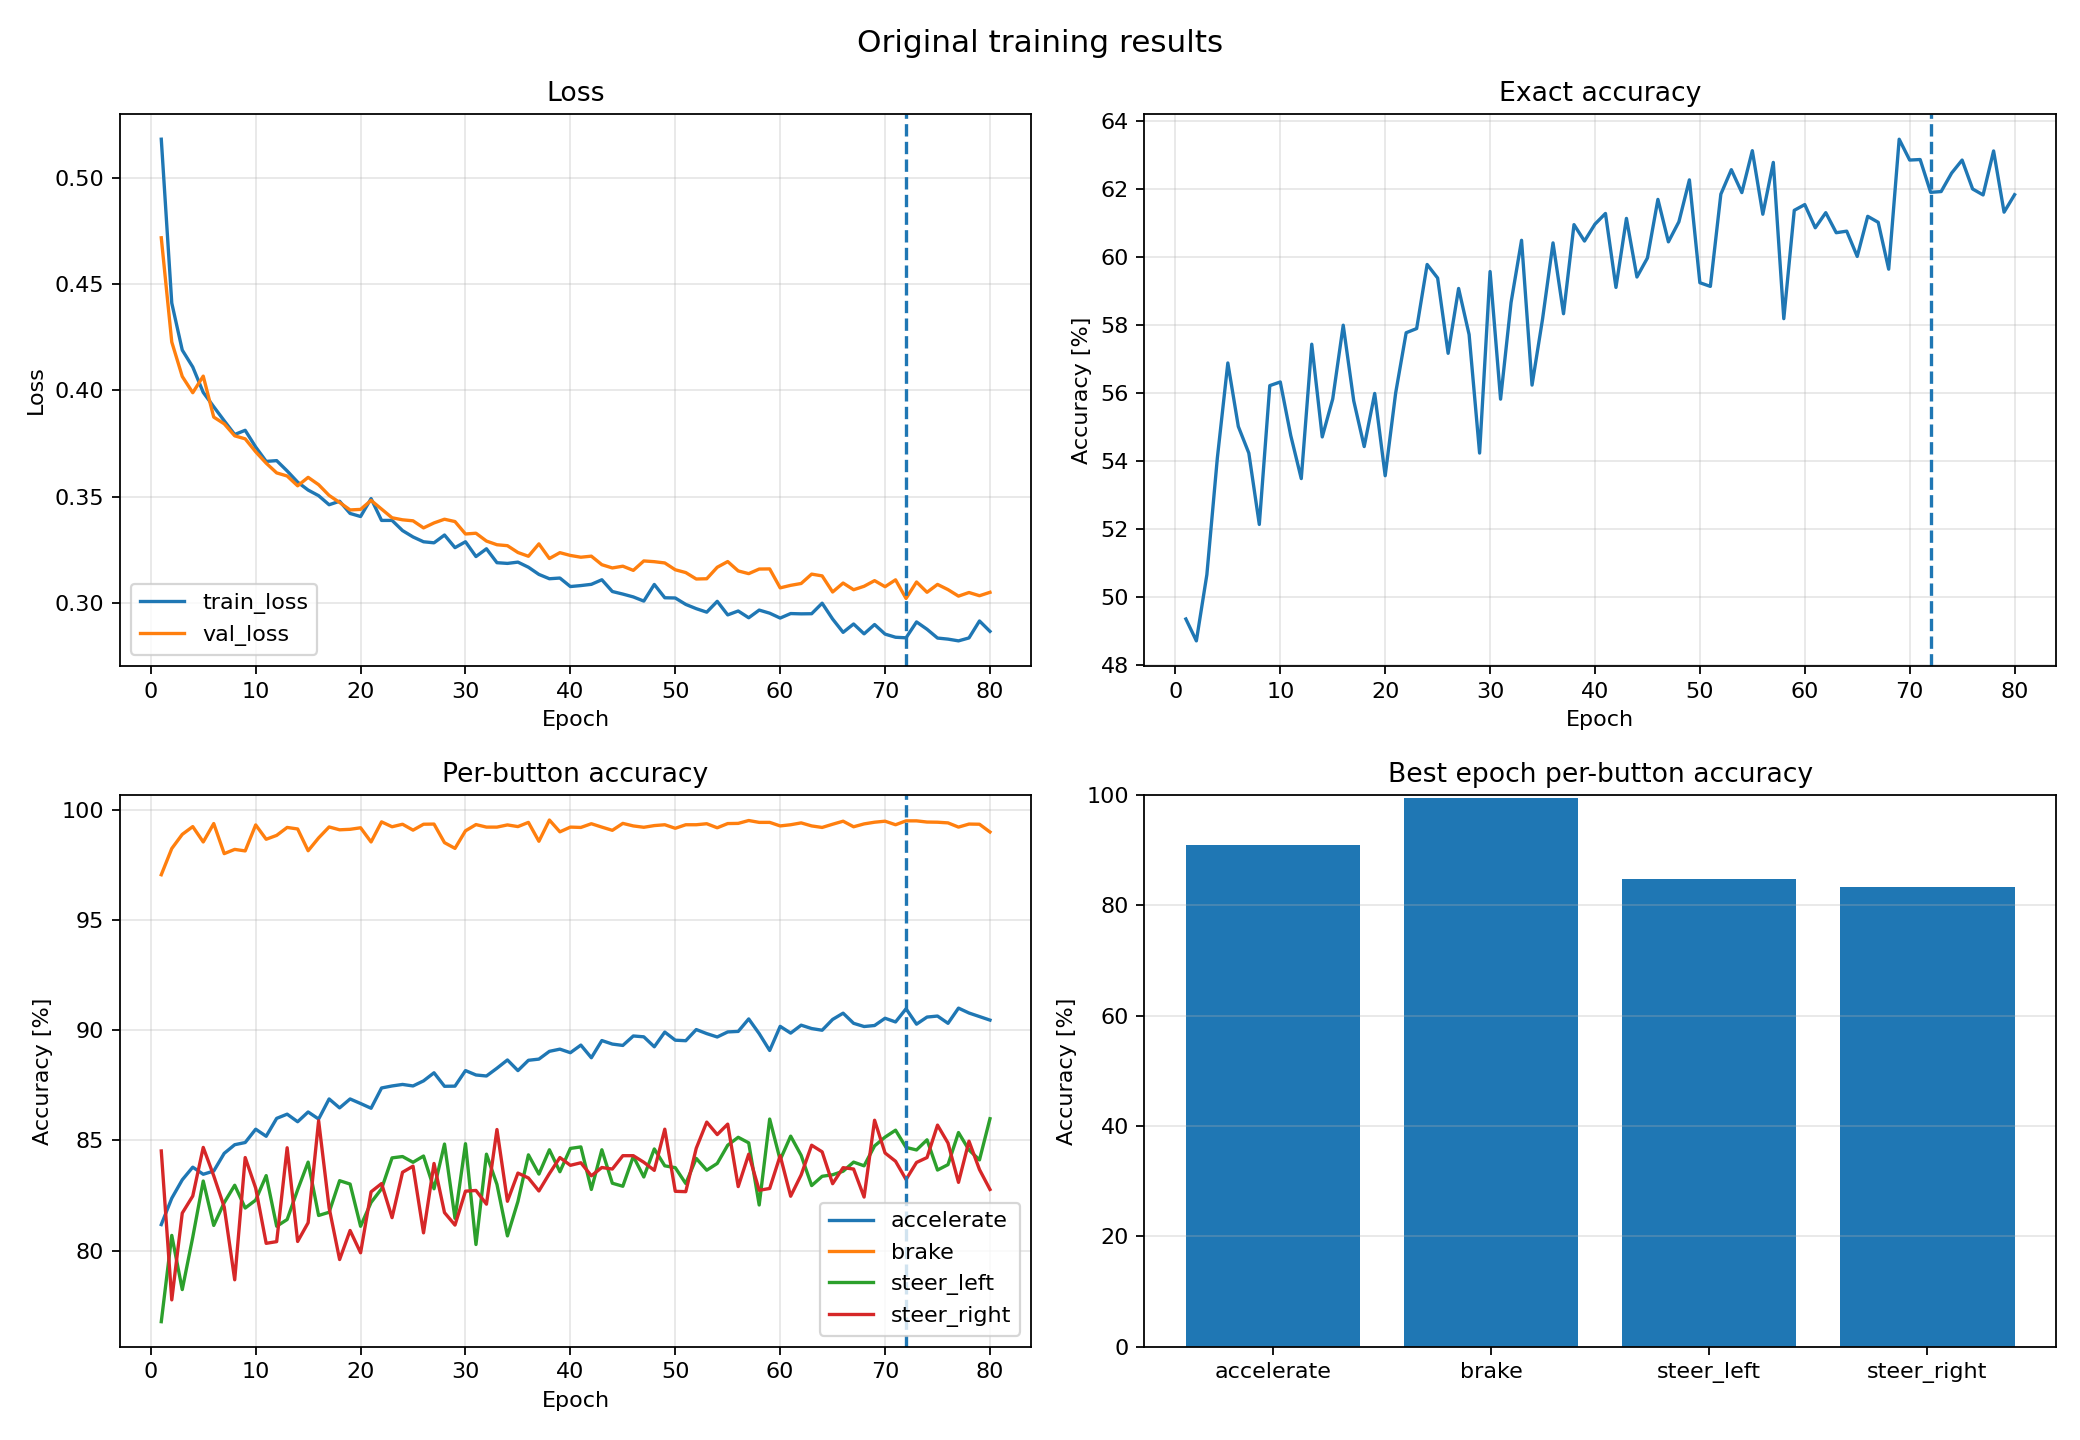
\includegraphics[width=\linewidth]{training_summary.png}
  \caption{Zbiorcze podsumowanie treningu modelu bazowego: strata, dokładność
  dokładna oraz dokładność per-przycisk wraz z wartościami w najlepszej epoce.}
  \label{fig:summary}
\end{figure}

\begin{figure}[H]
  \centering
  \begin{subfigure}{0.49\textwidth}
    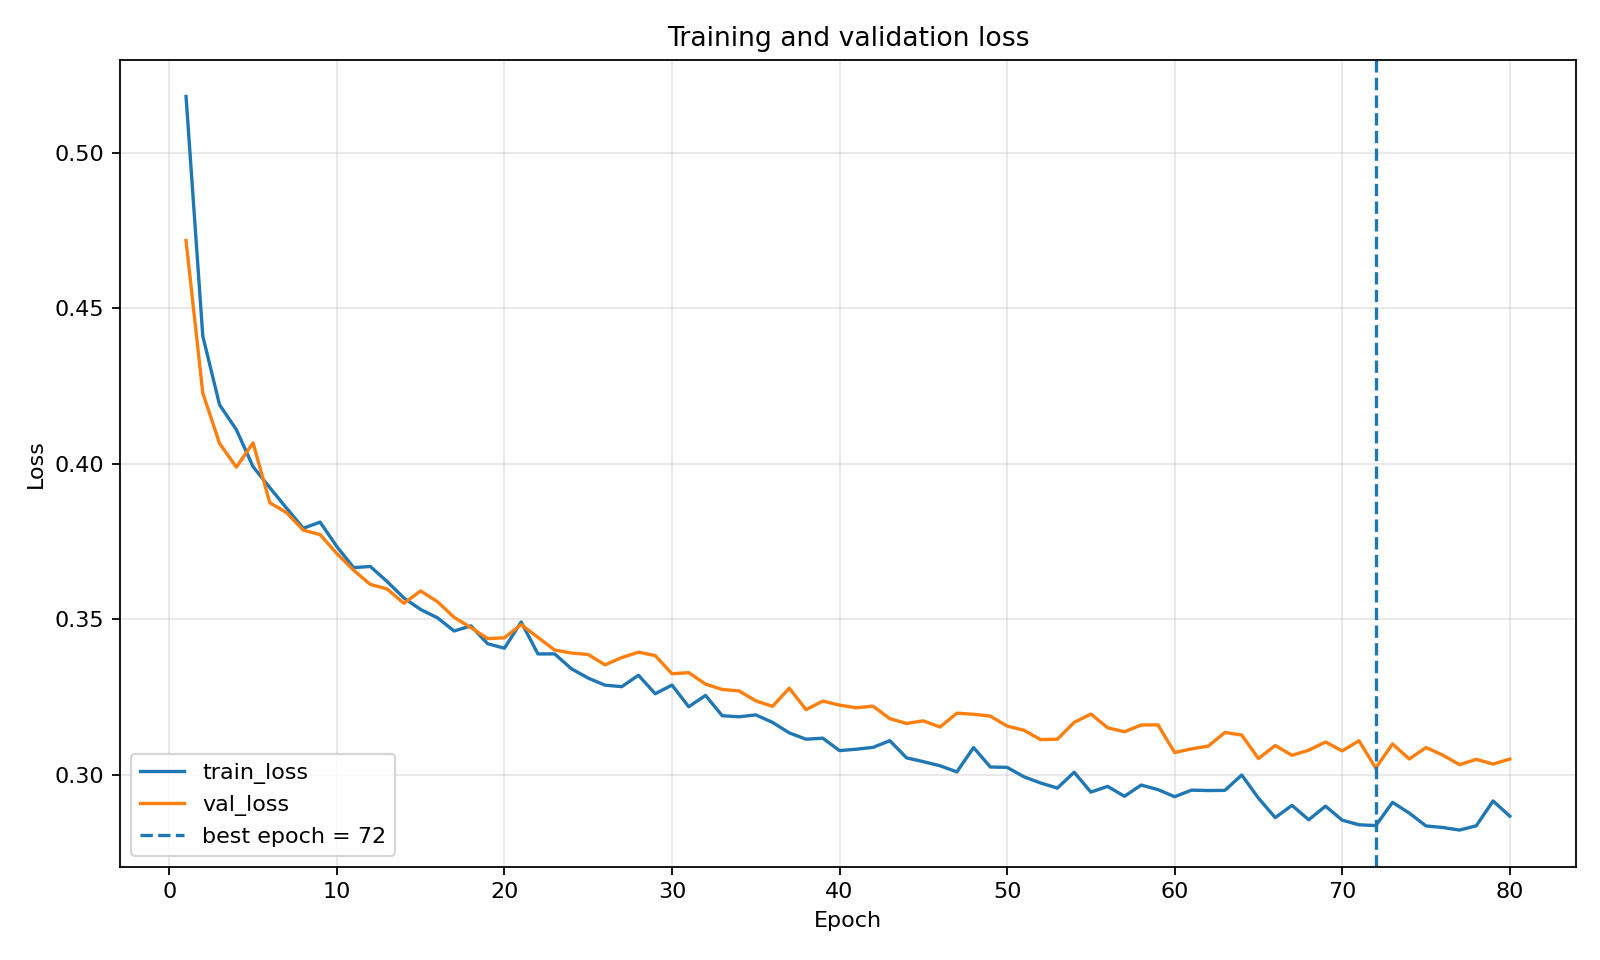
\includegraphics[width=\linewidth]{loss_curve.png}
    \caption{Strata treningowa i walidacyjna.}
    \label{fig:loss}
  \end{subfigure}\hfill
  \begin{subfigure}{0.49\textwidth}
    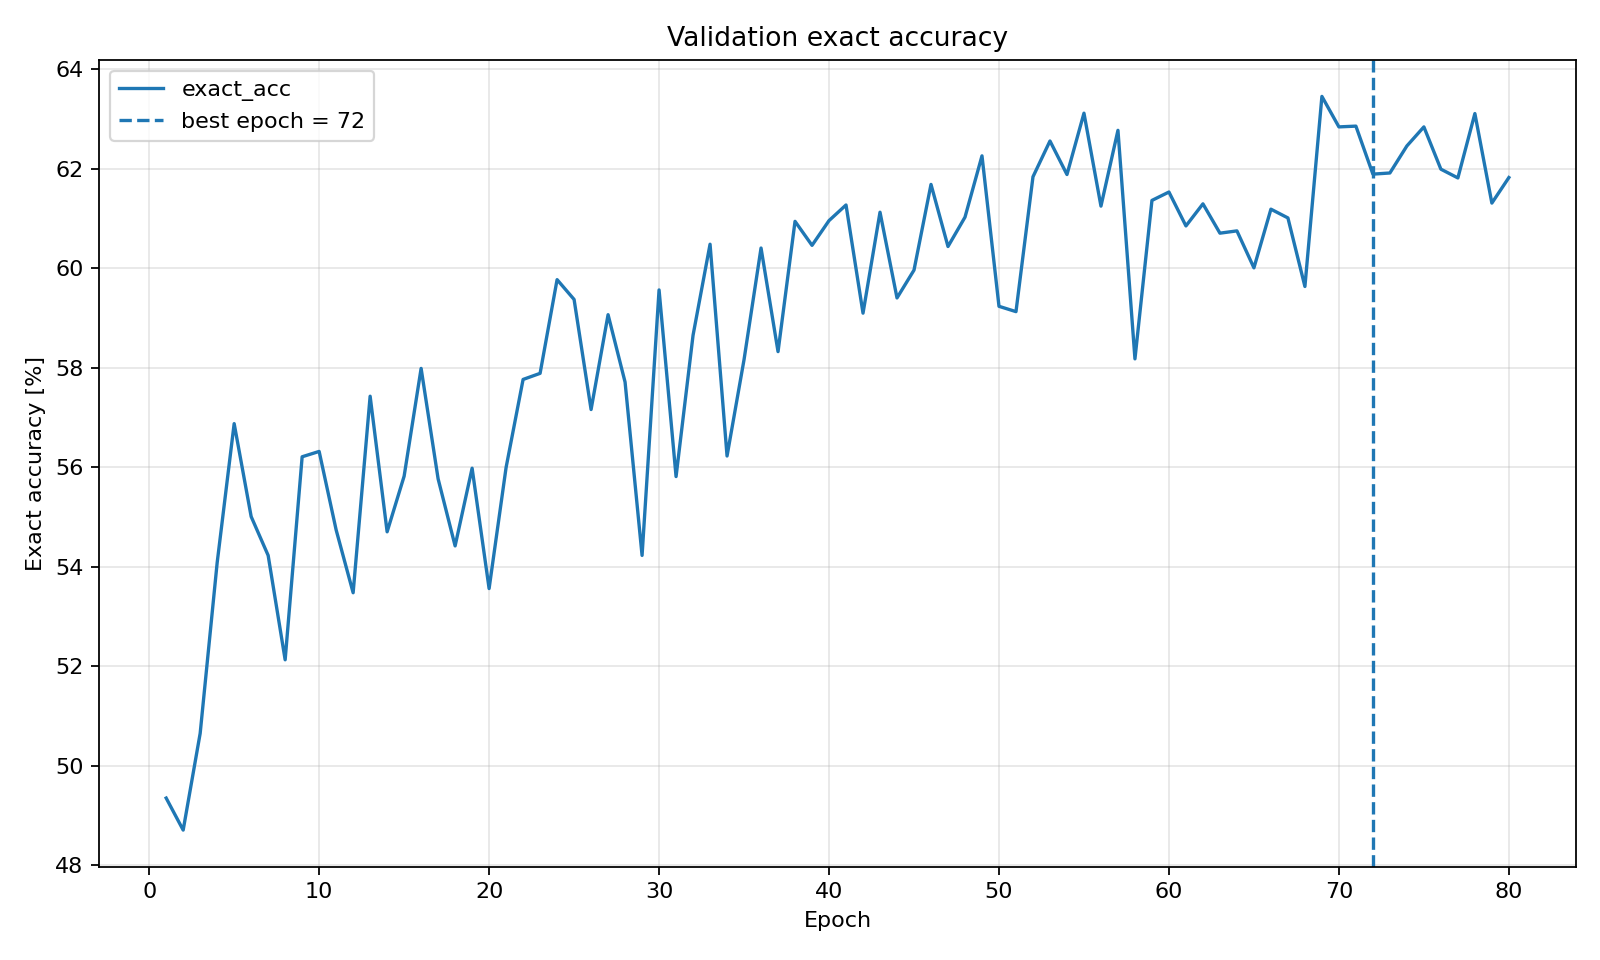
\includegraphics[width=\linewidth]{exact_accuracy_curve.png}
    \caption{Dokładność dokładna na walidacji.}
    \label{fig:exact}
  \end{subfigure}
  \caption{Krzywe uczenia. Strata walidacyjna stabilizuje się ok.~$0{,}30$, a
  dokładność dokładna rośnie do ok.~$62$--$63\%$. Niewielka różnica między stratą
  treningową a walidacyjną świadczy o umiarkowanym przeuczeniu.}
  \label{fig:krzywe}
\end{figure}

\subsection{Jakość poszczególnych akcji}

Dokładność per-przycisk (rysunki~\ref{fig:perbutton} i~\ref{fig:bestepoch})
pokazuje, że model najlepiej radzi sobie z hamowaniem (ok.~$99\%$ --- tu jednak
decyduje rzadkość klasy) oraz przyspieszaniem (ok.~$91\%$). Trudniejsze okazują się
skręty (ok.~$83$--$85\%$), co jest zgodne z intuicją: decyzja o skręcie wymaga
subtelniejszej interpretacji układu promieni niż decyzja o jeździe na wprost.

\begin{figure}[H]
  \centering
  \begin{subfigure}{0.55\textwidth}
    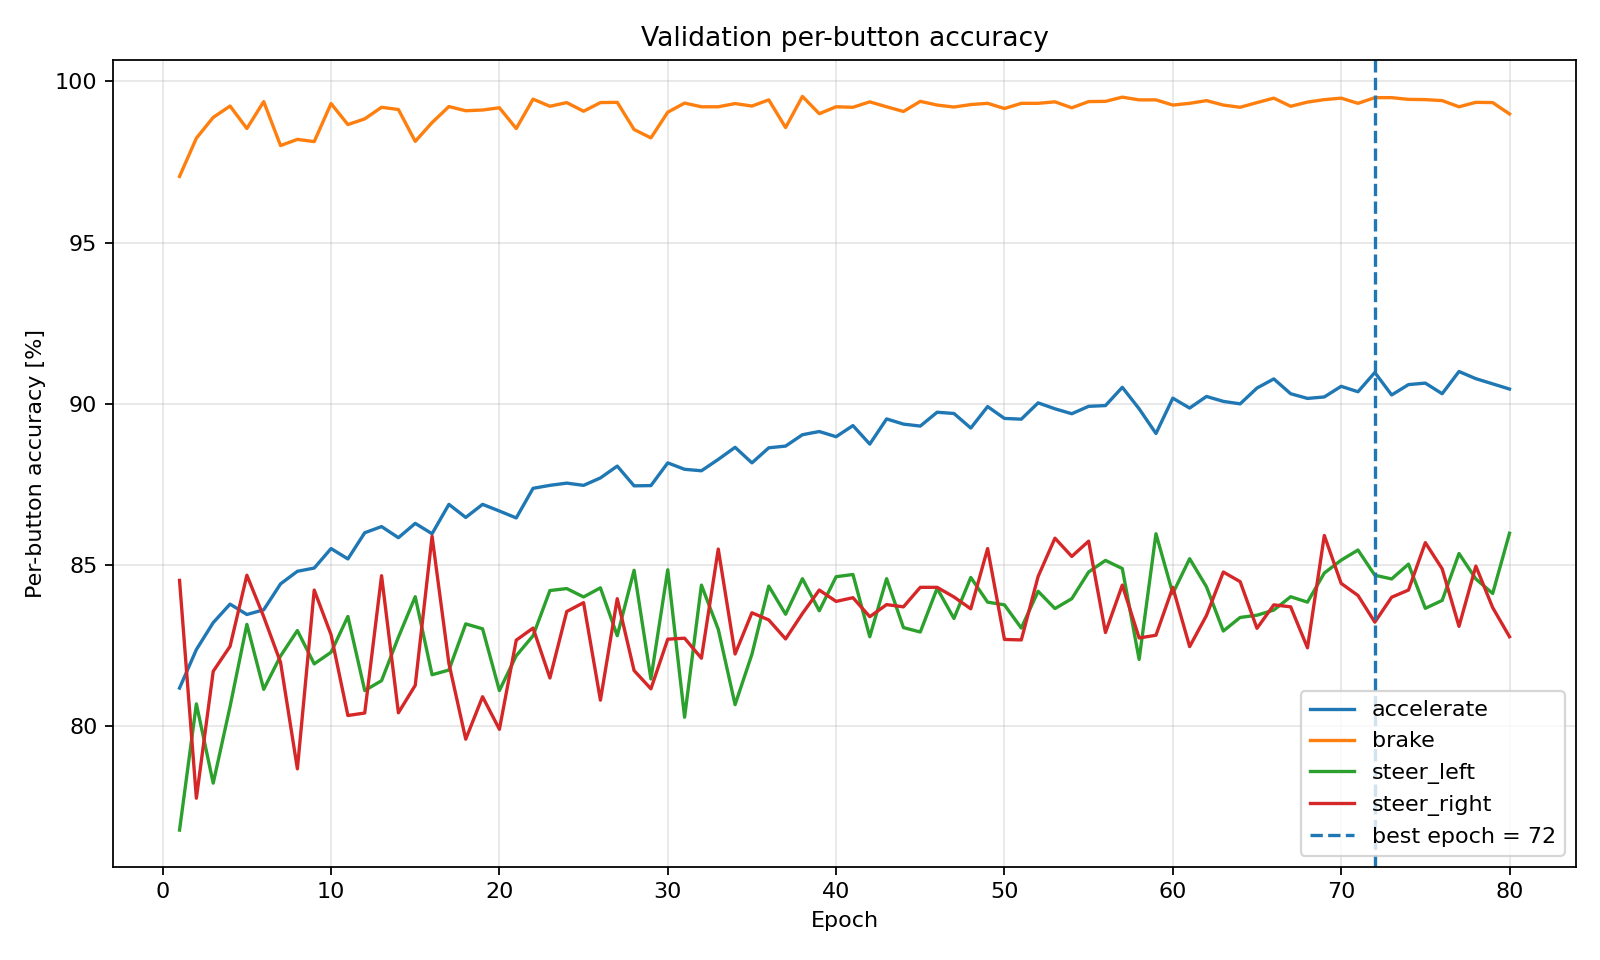
\includegraphics[width=\linewidth]{per_button_accuracy_curve.png}
    \caption{Dokładność per-przycisk w kolejnych epokach.}
    \label{fig:perbutton}
  \end{subfigure}\hfill
  \begin{subfigure}{0.43\textwidth}
    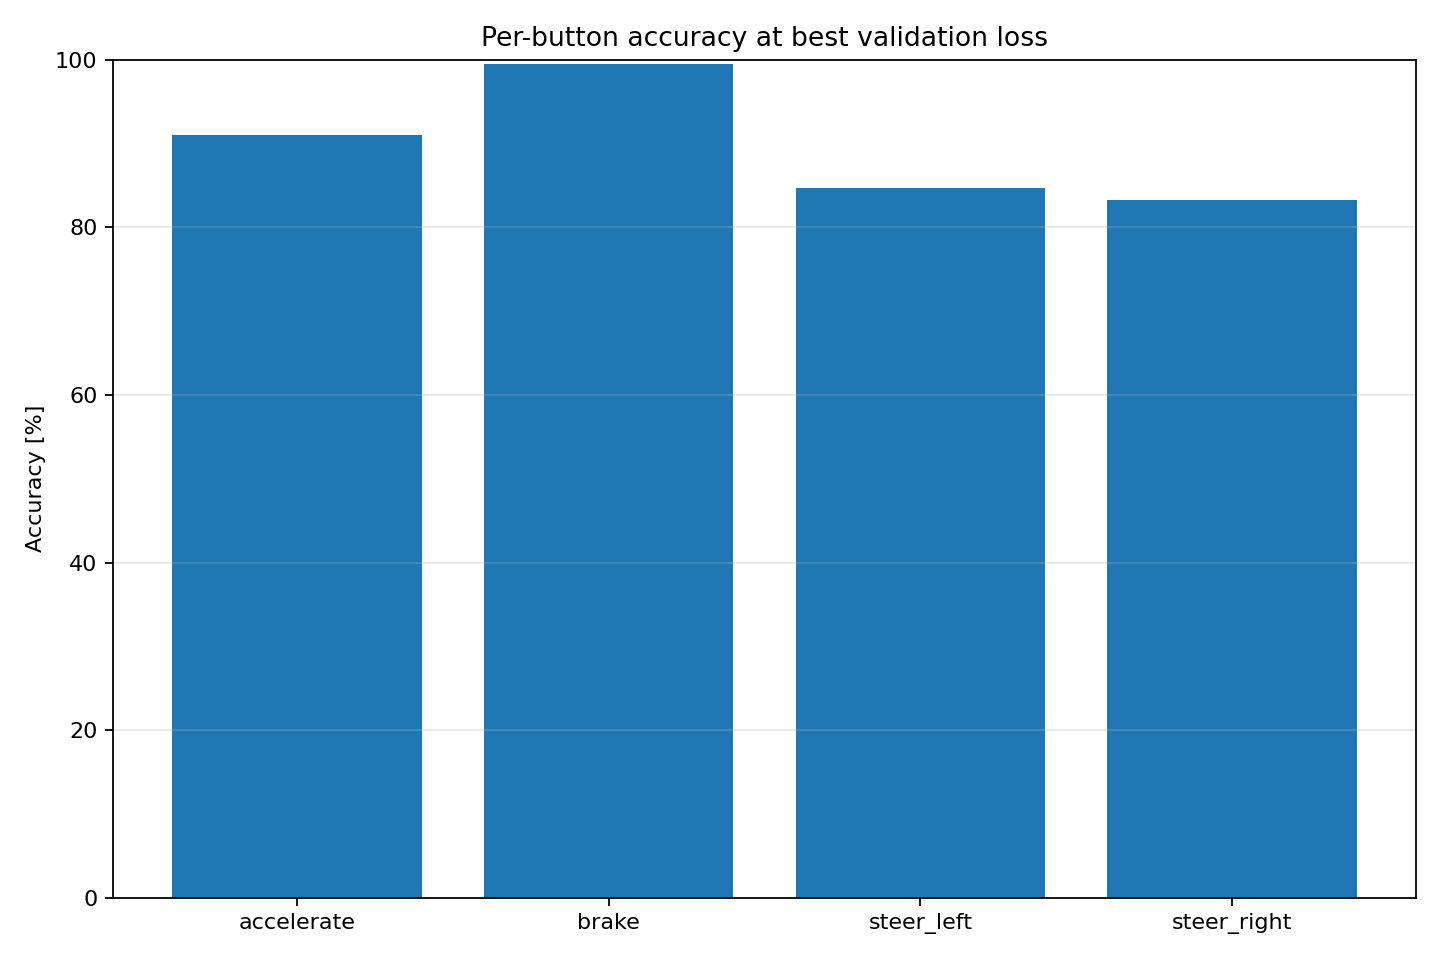
\includegraphics[width=\linewidth]{best_epoch_per_button_accuracy.png}
    \caption{Dokładność w najlepszej epoce.}
    \label{fig:bestepoch}
  \end{subfigure}
  \caption{Dokładność dla poszczególnych akcji. Skręt w lewo i w prawo to akcje
  najtrudniejsze do nauczenia.}
  \label{fig:perbutton_all}
\end{figure}

\subsection{Wyniki strojenia hiperparametrów}

Ranking konfiguracji według straty walidacyjnej (rysunek~\ref{fig:topval})
pokazuje, że wiele konfiguracji daje bardzo zbliżone wyniki (\texttt{val\_loss}
ok.~$0{,}077$--$0{,}080$), co świadczy o stabilności architektury względem
testowanych hiperparametrów. Ranking według dokładności dokładnej w trybie
runtime (rysunek~\ref{fig:topacc}) wskazuje najlepsze konfiguracje przekraczające
$70\%$ poprawnie odtworzonych pełnych zestawów akcji.

\begin{figure}[H]
  \centering
  \begin{subfigure}{0.49\textwidth}
    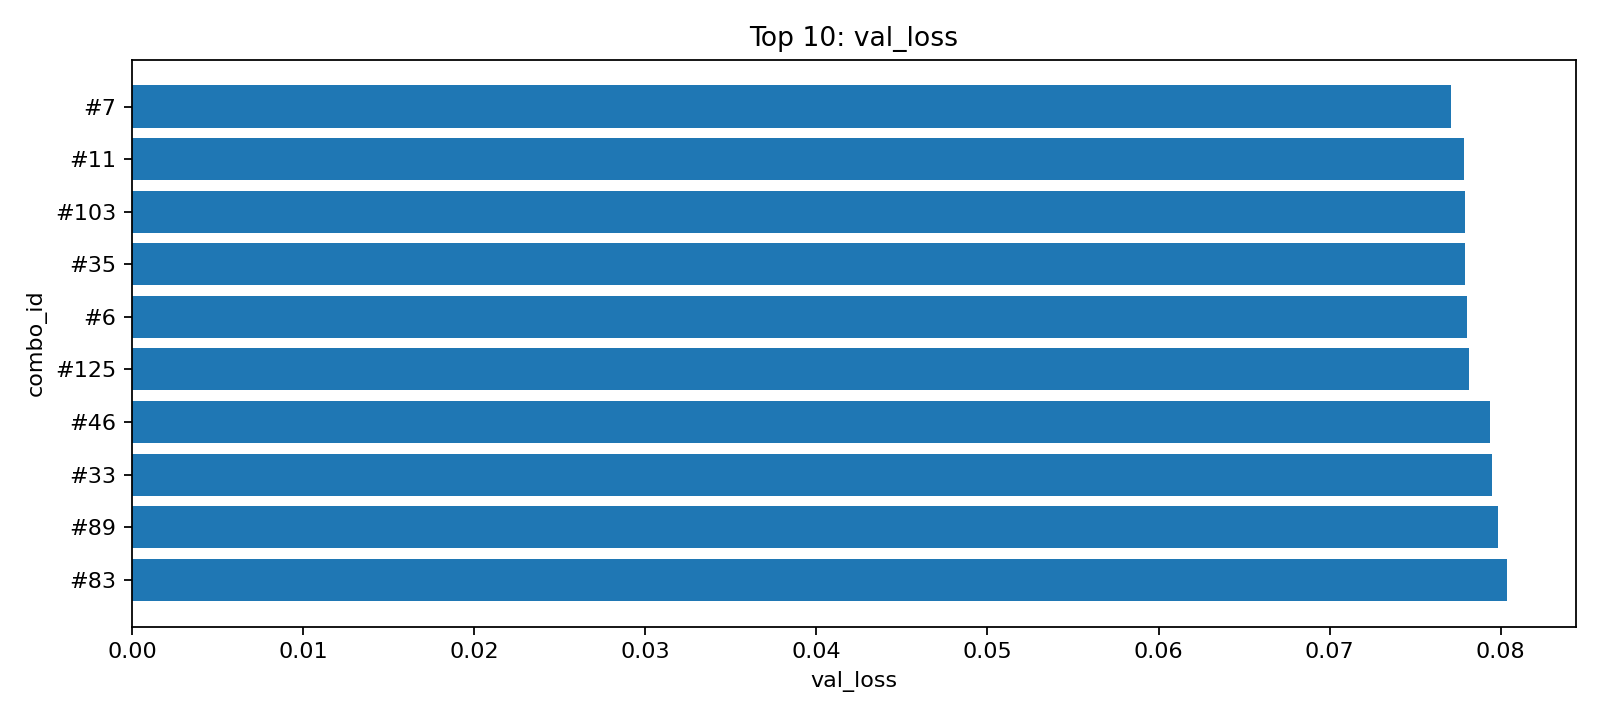
\includegraphics[width=\linewidth]{top_val_loss.png}
    \caption{Top~10 wg straty walidacyjnej.}
    \label{fig:topval}
  \end{subfigure}\hfill
  \begin{subfigure}{0.49\textwidth}
    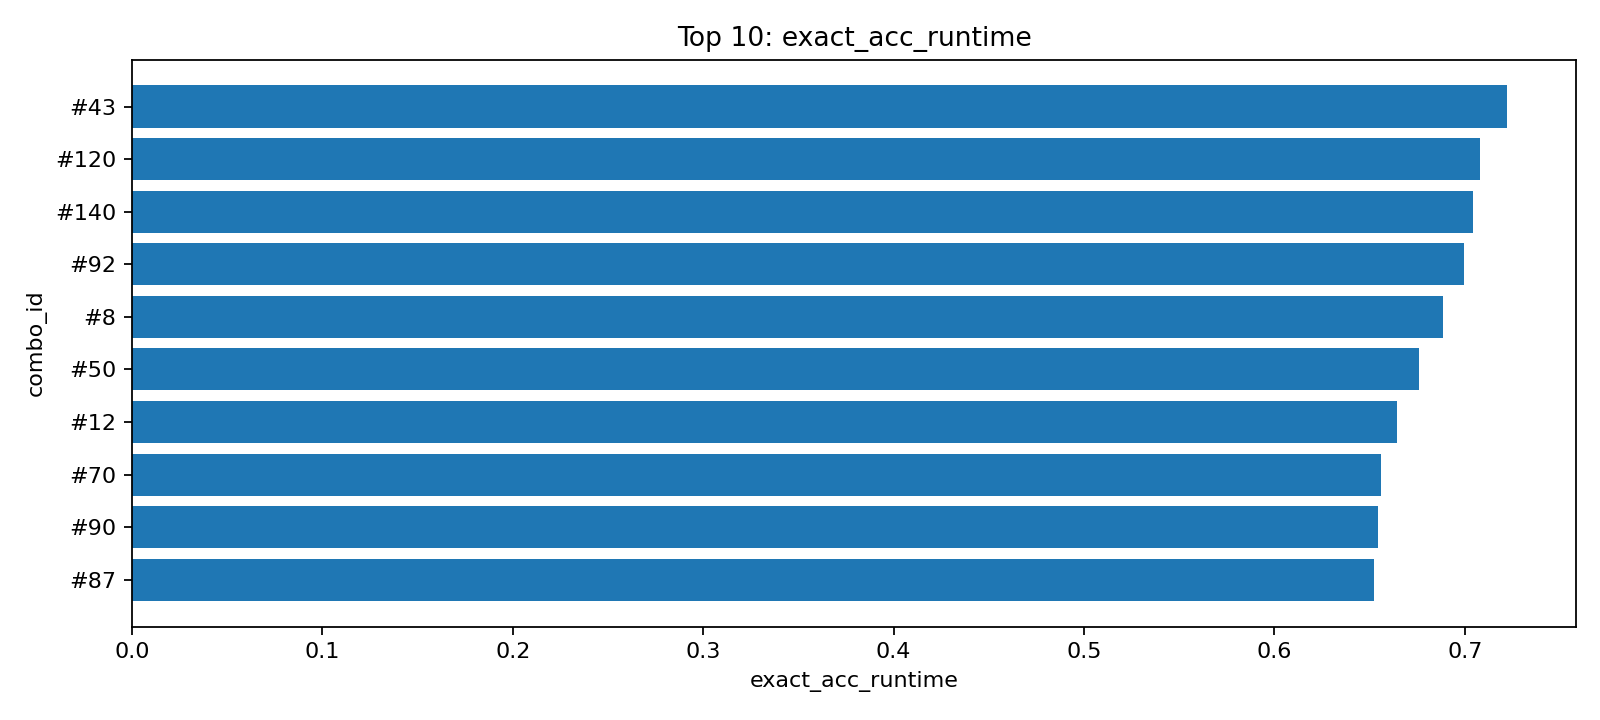
\includegraphics[width=\linewidth]{top_acc_runtime.png}
    \caption{Top~10 wg dokładności dokładnej (runtime).}
    \label{fig:topacc}
  \end{subfigure}
  \caption{Rankingi konfiguracji z przeszukiwania siatki hiperparametrów.}
  \label{fig:rankingi}
\end{figure}

Rysunek~\ref{fig:scatter} ilustruje zależność między uśrednioną miarą F1 (macro-F1)
a miarą F1 dla samego hamowania. Widać silną dodatnią korelację --- konfiguracje
dobre ,,ogólnie'' są zwykle dobre także w trudnej akcji hamowania, choć dla
najlepszych modeli pojawia się pewien kompromis między tymi metrykami.

\begin{figure}[H]
  \centering
  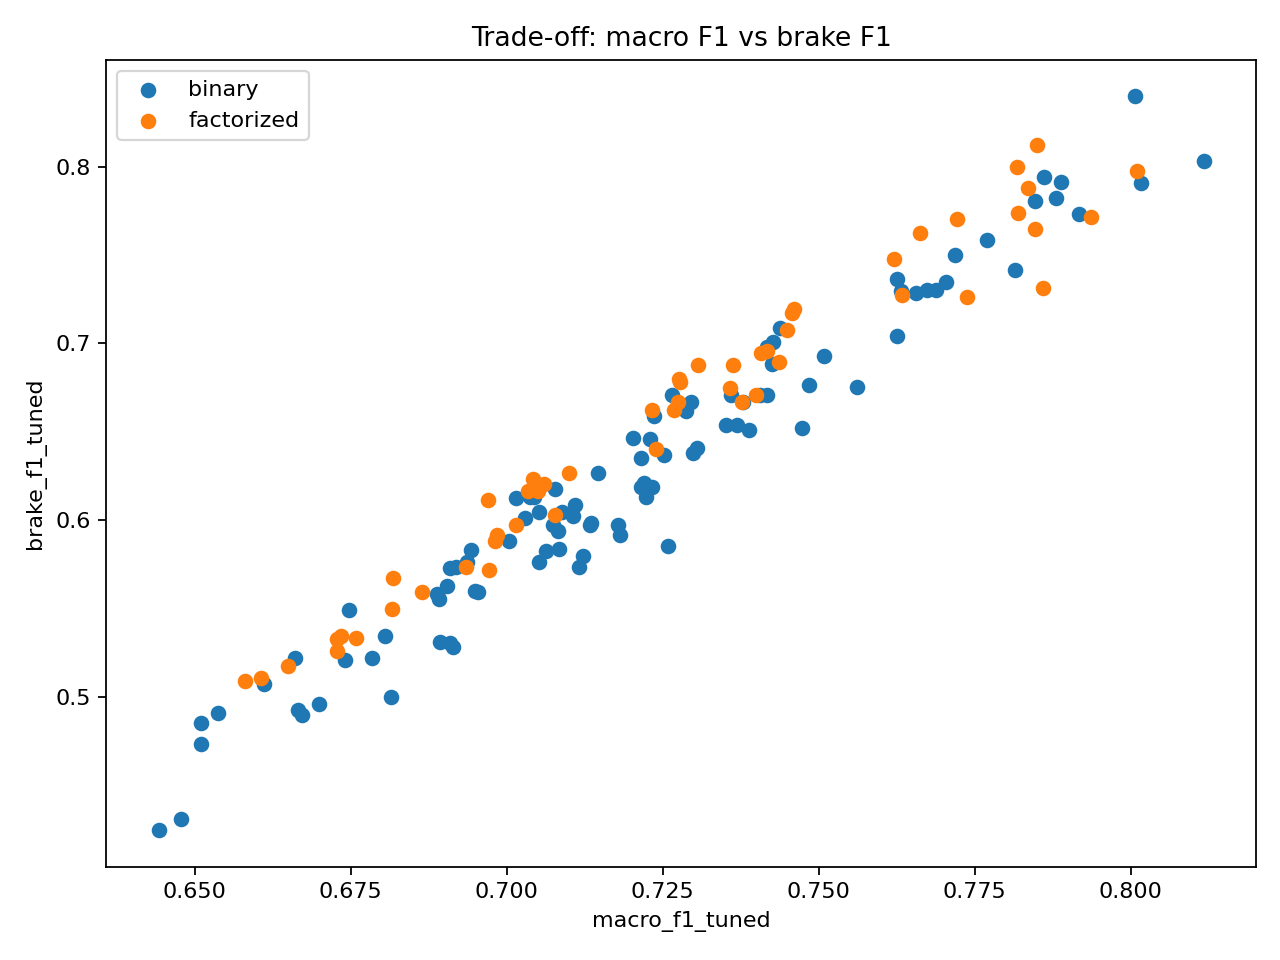
\includegraphics[width=0.7\linewidth]{scatter_macro_f1_vs_brake_f1.png}
  \caption{Kompromis między macro-F1 a F1 dla hamowania (po strojeniu progów).
  Każdy punkt to jedna konfiguracja modelu.}
  \label{fig:scatter}
\end{figure}

\subsection{Wybór najlepszego modelu}
\label{sec:najlepszy}

Na podstawie rankingu według straty walidacyjnej (rysunek~\ref{fig:topval})
jako najlepszą wybrano konfigurację \textbf{nr~7}. Wyróżnia się ona najniższą
stratą walidacyjną oraz najwyższym macro-F1 (po dostrojeniu progów). Jej kluczowe
hiperparametry oraz osiągnięte wyniki zestawiono w tabeli~\ref{tab:best}.

\begin{table}[H]
  \centering
  \caption{Hiperparametry i wyniki najlepszej konfiguracji (model~nr~7).}
  \label{tab:best}
  \begin{tabular}{ll}
    \toprule
    \textbf{Parametr / metryka} & \textbf{Wartość} \\
    \midrule
    Struktura sieci (\texttt{hidden\_layers}) & \texttt{256,256,128,64} \\
    Aktywacja                                  & \texttt{relu} \\
    Normalizacja                               & \texttt{batch} \\
    Dropout                                    & $0{,}0$ \\
    Współczynnik uczenia (\texttt{lr})         & $10^{-3}$ \\
    Regularyzacja (\texttt{weight\_decay})     & $10^{-3}$ \\
    Rozmiar wsadu (\texttt{batch\_size})       & $2048$ \\
    Limit wagi klasy (\texttt{pos\_weight\_cap}) & $10$ \\
    Progi decyzyjne (acc, brake, left, right)  & $[0{,}45,\ 0{,}65,\ 0{,}60,\ 0{,}60]$ \\
    \midrule
    Strata walidacyjna (\texttt{val\_loss})    & $0{,}0771$ \\
    macro-F1 (progi runtime)                   & $0{,}7492$ \\
    macro-F1 (progi dostrojone)                & $0{,}8117$ \\
    F1 hamowania (progi dostrojone)            & $0{,}8031$ \\
    \bottomrule
  \end{tabular}
\end{table}

\subsection{Porównanie z modelem bazowym}

Najlepsza konfiguracja osiąga niższą stratę walidacyjną ($0{,}0771$) i wyższe
macro-F1 niż model bazowy, przy zachowaniu wysokiej skuteczności hamowania
(F1 $\approx 0{,}80$). Warto zauważyć, że dostrojenie progów decyzyjnych podnosi
macro-F1 z $0{,}7492$ (progi domyślne) do $0{,}8117$ --- to potwierdza, że
\textbf{łączne} dostrojenie wag sieci oraz progów daje większy zysk niż optymalizacja
pojedynczego hiperparametru, a celem jest sprawny kierowca, a nie minimalizacja
jednej liczby.

% =====================================================================
\section{Wdrożenie modelu w grze}
\label{sec:wdrozenie}

Wytrenowany model eksportowany jest do formatu \textbf{ONNX} i ładowany w grze
przez klasę \texttt{NeuralDriver} (biblioteka ONNX Runtime). W każdej klatce gra:
\begin{enumerate}[noitemsep]
  \item buduje 81-elementowy wektor wejściowy ze stanu pojazdu
        (\texttt{BuildAIInput\allowbreak From\allowbreak GameState}),
  \item uruchamia model i otrzymuje 4 logity,
  \item nakłada sigmoidę, uzyskując prawdopodobieństwa,
  \item stosuje progi i zasady decyzyjne (priorytet hamowania, wybór jednego
        kierunku skrętu), zamieniając prawdopodobieństwa na sterowanie.
\end{enumerate}

\noindent\begin{minipage}{\linewidth}
\begin{lstlisting}[style=cpp,caption={Zamiana prawdopodobieństw na sterowanie w grze (fragment \texttt{NeuralDriver.cpp}). Progi dostosowano do wartości z grid search.}]
Controls NeuralDriver::PredictControls(const GameState& state) {
    std::vector<float> probs = PredictProbabilities(state);
    float pAccelerate = probs[0], pBrake = probs[1];
    float pSteerLeft = probs[2], pSteerRight = probs[3];

    Controls controls{};
    if (pBrake > 0.65f)           controls.brake = 1.0f;        // priorytet hamulca
    else if (pAccelerate > 0.45f) controls.accelerate = 1.0f;

    float steeringThreshold = 0.60f;                            // left/right z grid search
    if (pSteerLeft > steeringThreshold || pSteerRight > steeringThreshold) {
        if (pSteerLeft > pSteerRight) controls.steerLeft = 1.0f;
        else                          controls.steerRight = 1.0f;
    }
    return controls;
}
\end{lstlisting}
\end{minipage}

Progi decyzyjne po stronie C++ zostały \textbf{dostosowane do wartości wyłonionych
w grid search} dla najlepszego modelu (rozdział~\ref{sec:najlepszy}),
tj.\ $[0{,}45,\ 0{,}65,\ 0{,}60,\ 0{,}60]$ odpowiednio dla gazu, hamulca oraz skrętu
w lewo i prawo. Dzięki temu zachowanie modelu w grze odpowiada wynikom uzyskanym na
zbiorze walidacyjnym. Przełączanie między kierowcą-człowiekiem a kierowcą-AI odbywa
się w grze klawiszem \texttt{M}.

% =====================================================================
\section{Analiza błędów i ograniczenia}
\label{sec:bledy}

\begin{itemize}
  \item \textbf{Najczęściej mylone akcje:} skręt w lewo i skręt w prawo. Model
        bywa niezdecydowany w sytuacjach symetrycznych, gdy oba kierunki mają
        zbliżone prawdopodobieństwo --- stąd reguła wyboru jednego (silniejszego)
        kierunku.
  \item \textbf{Imitacja, nie optymalizacja jazdy:} model uczy się odwzorowywać
        decyzje gracza, więc dziedziczy jego błędy i nie eksploruje lepszych
        strategii niewystępujących w danych.
  \item \textbf{Zależność od jakości danych:} sytuacje rzadkie na torze (ostre
        zakręty, cofanie) są słabo reprezentowane, co obniża skuteczność modelu
        w takich momentach.
  \item \textbf{Wyciek informacji:} przy losowym podziale na poziomie pojedynczych
        klatek kolejne, niemal identyczne klatki tego samego przejazdu mogą trafić
        do treningu i walidacji jednocześnie. Podział grupowy po przejazdach
        ogranicza ten efekt.
\end{itemize}

% =====================================================================
\section{Wnioski i kierunki dalszych prac}
\label{sec:wnioski}

\paragraph{Wnioski.}
\begin{itemize}[noitemsep]
  \item Udało się \textbf{nauczyć komputer sterowania samochodem} w grze 2D ---
        sieć neuronowa na podstawie 20 promieni i prędkości podejmuje sensowne
        decyzje sterujące w czasie rzeczywistym.
  \item Kluczowe okazały się: ważenie rzadkich klas (\texttt{pos\_weight}) oraz
        strojenie progów decyzyjnych, a nie samo dostrajanie wag sieci.
  \item Najtrudniejszym elementem jazdy są skręty; hamowanie, mimo rzadkości,
        jest dobrze rozpoznawane dzięki ważeniu klas.
  \item Przeszukiwanie hiperparametrów potraktowano jako narzędzie poprawy
        kierowcy --- różnice między najlepszymi konfiguracjami są niewielkie, co
        świadczy o stabilności rozwiązania.
\end{itemize}

\paragraph{Dalsze prace.}
\begin{itemize}[noitemsep]
  \item zastosowanie \textbf{uczenia ze wzmocnieniem} (RL), aby model optymalizował
        czas przejazdu, a nie jedynie naśladował gracza,
  \item dodanie informacji o \textbf{historii} (kilka poprzednich klatek lub sieć
        rekurencyjna) dla płynniejszego sterowania,
  \item zbieranie danych z wielu torów i wielu graczy w celu lepszej generalizacji,
  \item rejestrowanie identyfikatora przejazdu (\texttt{episode\_id}) dla rzetelnego
        podziału grupowego i uczciwszej oceny.
\end{itemize}

% =====================================================================
\begin{thebibliography}{9}
\bibitem{pytorch} A. Paszke i in., \emph{PyTorch: An Imperative Style,
High-Performance Deep Learning Library}, NeurIPS, 2019.
\bibitem{sklearn} F. Pedregosa i in., \emph{Scikit-learn: Machine Learning in
Python}, JMLR, 2011.
\bibitem{onnx} ONNX Runtime, \emph{Open Neural Network Exchange Runtime},
\url{https://onnxruntime.ai}.
\bibitem{raylib} R. Santamaria, \emph{raylib --- a simple and easy-to-use library
to enjoy videogames programming}, \url{https://www.raylib.com}.
\end{thebibliography}

\end{document}
